\documentclass[../main]{subfiles}

\begin{document}

Let $\base$ denote a fixed topological space, which will be called the \defemph{base space}\index{base space}.


\begin{definition}\label{def:02.01}
A real \defemph{vector bundle}\index{vector bundle} $\xi$ over $\base$ consists of the following:
\begin{enumerate}[label = \arabic*)]

    \item A topological space $\total=\total(\xi)$ called the \defemph{total space}\index{total space $E(\xi)$}.
    
    \item A (continuous) map $\pi:\total\varrightarrow{}\base$ called the \defemph{projection map}\index{projection map}.
    
    \item For each $b\in\base$, the structure of a vector space\footnote{
    To be more precise, this vector space structure could be specified by giving the subset of $\bR\times\bR\times \total \times \total \times \total$ consisting of all 5-tuples $(t_1,t_2,e_1,e_2,e_3)$ with
    \[\pi(e_1)=\pi(e_2)=\pi(e_3) \text { and }e_3=t_1e_1+t_2e_2\]} over the real numbers in the set $\pi\inv(b)$.
    
\end{enumerate}
\end{definition}


These must satisfy the following restriction:

Condition of \defemph{local triviality}\index{local triviality}. For each point $p\in\base$, there should exist a neighborhood $U\subset\base$, and integer $n\ge0$, and a homeomorphism \newline $h:U\times\bR^n\varrightarrow{}\pi\inv(U)$ so that, for each $b\in U$, the correspondence $x\mapsto h(b,x)$ defines an isomorphism between the vector space $\bR^n$ and the vector space $\pi\inv(b)$.

Such a pair $(U,h)$ will be called a \defemph{local coordinate system for $\xi$ about $b$}\index{local coordinate system}. If it is possible to choose $U$ equal to the entire base space, then $\xi$ will be called a \defemph{trivial bundle}\index{trivial bundle $\trivialbundle^n$}.

The vector space $\pi\inv(b)$ is called the \defemph{fiber over}\index{fibre space $F_b$} $b$. It may be denoted by $F_b$ or $F_b(\xi)$. Note that $F_b$ is never vacuous, although it may consist of a single point. The dimension $n$ of $F_b$ is allowed to be a (locally constant) function of $b$; but in most cases of interest this function is constant. One then speaks of an \defemph{$n$-plane bundle}\index{n-plane bundle@$n$-plane bundle}, or briefly an \defemph{$\bR^n$-bundle}\index{Rn-bundle@$\bR^n$-bundle}\index{real vector bundle}.

The concept of a \defemphi{smooth vector bundle}\index{vector bundle!\indexline smooth} can be defined similarly. One requires that $\base$ and $\total$ be smooth manifolds, that $\pi$ be a smooth map, and that, for each $b\in\base$ there exist a local coordinate system $(U, h)$ with $b \in U$ such that $h$ is a diffeomorphism\index{diffeomorphism}.


\begin{remark*}
An $\bR^n$-bundle is a very special example of a \defemphi{fibre bundle}.
(See \cite{steenrodwhitehead1951}.) In Steenrod's terminology an $\bR^n$-bundle is a
fiber bundle with fiber $\bR^n$ and with the full linear group $\GL_n(\bR)$\index{linear group $\GL_n$!\indexline real} in $n$
variables as structural group\index{structural group}.
\end{remark*}


Now consider two vector bundles $\xi$ and $\eta$ over the same base space $\B$.


\begin{definition}\label{def:02.02}
$\xi$ is \defemph{isomorphic}\index{isomorphic (vector bundles)} to $\eta$, written $\xi \cong \eta$, if there exists
a homeomorphism \[f:\total(\xi)\varrightarrow{}\total(\eta)\] between the total spaces which maps each vector space $F_b(\xi)$ isomorphically onto the corresponding vector space $F_b(\eta)$.
\end{definition}


\begin{example}\label{ex:02.01}
The trivial bundle with total space $\B \times \bR^n$, with 
projection map $\pi(b, x) = b$, and with the vector space structures in the fibers defined by
\[t_1(b,x_1) + t_2(b,x_2) = (b,t_1x_1 + t_2x_2)\]
will be denoted by $\trivialbundle^n_{\B}$. Note that a $\bR^n$-bundle over ${\B}$ is trivial
if and only if it is isomorphic to $\trivialbundle^n_{{\B}}$.
\end{example}


\begin{example}\label{ex:02.02}
The \defemph{tangent bundle $\tangentBundle{M}$}\index{tangent bundle $\tangentbundle{M}$}
 of a smooth manifold $M$. The
total space of $\tangentBundle{M}$ is the manifold $\tangentTS M$ consisting of all pairs $(x,v)$ with
$x \in M$ and $v$ tangent to $M$ at $x$. The projection map $\pi:\tangentTS M \varrightarrow{} M$
is defined by $\pi(x, v) = x$; and the vector space structure in $\pi\inv(x)$ is defined by
\[t_1(x,v_1) + t_2(x,v_2) = (x,t_1v_1 + t_2v_2). \]
The local triviality condition is not difficult to verify. Note that $\tangentBundle{M}$ is
an example of a smooth vector bundle.
\end{example}


If $\tangentBundle{M}$ is a trivial bundle, then the manifold $M$ is called \defemphi{parallelizable}.
For example, suppose that $M$ is an open subset of $\bR^n$. Then $\tangentTS M$ is
equal to $M \times \bR^n$, and $M$ is clearly parallelizable.

The unit $2$-sphere $\Sphere^{2}\subset \bR^3$ provides an example of a manifold which
is not parallelizable. (Compare \ref{prob-2-B}.) In fact we will see in \S\ref{ch:9}
that a parallelizable manifold must have Euler characteristic\index{Euler characterist or Euler number} zero, whereas
the $2$-sphere has Euler characteristic $+2$. (See Proposition \ref{pro:09.03} and Lemma~\ref{lem:11.6}.)


\begin{example}\label{ex:02.03}
The normal bundle\index{normal bundle} $\normalbundle{M}$ of a smooth manifold $M \subset \bR^n$ is
obtained as follows. The total space
$\total \subset M \times \bR^n$
is the set of all pairs $(x, v)$ such that $v$ is orthogonal to the tangent
space $\tangentspace Mx$ . The projection map $\pi: \total \varrightarrow{} M$ and the vector space 
structure in $\pi\inv(x)$ are defined, as in Examples \ref{ex:02.01}, \ref{ex:02.02}, by the formulas
\[\pi(x, v) = x,
\quad t_1(x, v_1) + t_2(x, v_2) = (x, t_1v_1 + t_2v_2).\]
The proof that $\normalbundle{M}$ satisfies
the local triviality condition will be deferred until \ref{cor:03.04}.
\end{example}


\begin{example}\label{ex:02.04}
The \defemph{real projective space}\index{projective space!\indexline real $\projective^n$} $\projective^{n}$ can be defined\footnote{
Alternatively, $\projective^{n}$ can be defined as the set of lines through the origin in $\bR^{n+1}$.
(Compare \ref{prob:1-B}.) This amounts to the same thing since every
such line cuts $S^{n}$ in two antipodal points.}
as the set of all unordered pairs $\brc{x, -x}$ where $x$ ranges over the unit sphere
$S^{n} \subset\bR^{n+1}$; and is topologized as a quotient space of $S^{n}$.

Let $\total(\tautological^1_n)$ be the subset of $\projective^{n}\times \bR^{n+1}$ consisting of all pairs
$(\brc{\pm x}, v)$ such that the vector $v$ is a multiple of $x$. Define $\pi: \total(\tautological^1_n)\varrightarrow{} \projective^{n}$
by $\pi(\brc{\pm x} , v) = \brc{\pm x}$. Thus each fiber $\pi\inv(\brc{\pm x})$ can be identified with
the line through $x$ and $-x$ in $\bR^{n+1}$. Each such line is to be given its
usual vector space structure. The resulting vector bundle $\tautological^1_n$ will be
called the \defemph{canonical line bundle}\index{cannonical bundle!\indexline line $\tautological^1$} over $\projective^{n}$.


\begin{proof}
[\textsc{Proof that $\tautological^1_n$ is locally trivial.}] Let $U \subset S^{n}$ be any open set which
is small enough so as to contain no pair of antipodal points, and let $U_1$
denote the image of $U$ in $\projective^{n}$. Then a homeomorphism $h:U_1\times \bR\varrightarrow{}\pi\inv(U_1)$
is defined by the requirement that $h(\brc{\pm x},t)=(\brc{\pm x},tx)$ for each $(x, t)\in U \times \bR$. Evidently $(U_1,h)$ is a local coordinate system; hence $\tautological^1_n$ is locally trivial.
\end{proof}

\end{example}


\begin{theorem}\label{thm:02.01}
The bundle $\tautological^1_n$ over $\projective^{n}$ is not trivial, for $n \geq 1$.
\end{theorem}

\begin{proof}
This will be proved by studying cross-sections of $\tautological_n^1$

\begin{definition}\label{def:02.03}

A \defemphi{cross-section} of a vector bundle $\xi$ with base space
${\B}$ is a continuous function $s:{\B}\varrightarrow{} \total(\xi)$ which takes each $b \in {\B}$ into the corresponding fiber $F_b (\xi)$. Such a cross-section is \defemph{nowhere zero} if $s(b)$ is a non-zero vector of $F_b (\xi)$ for each $b$. 

(A cross-section of the tangent bundle of a smooth manifold $M$ is
usually called a \defemphi{vector field} on $M$.)
	
\end{definition}


Evidently a trivial $\bR^1$-bundle possesses a cross-section which is nowhere zero. We will see that the bundle $\tautological^1_n$ has no such cross-section.

Let $s:\projective^{n}\varrightarrow{} \total(\tautological^1_n)$
be any cross-section, and consider the composition
\[S^{n}\varrightarrow{}\projective^{n}\varrightarrow s \total(\tautological^1_n)\]
which carries each $x \in S^{n}$ to some pair
\[\br{\brc{\pm x},t(x)x}\in \total(\tautological^1_n)\]
Evidently $t(x)$ is a continuous real valued function of $x$, and $t(-x)=-t(x)$.
Since $S^{n}$ is connected, it follows from the intermediate value theorem
that $ t(x_0) = 0 $ for some $x_0$. Hence $s(\brc{\pm x_0})=(\brc{\pm x_0},0)$. This completes the proof.\end{proof}

It is interesting to take a closer look at the space $\total(\tautological^1_n)$ for the 
special case $n = 1$. In this case each point $e = (\brc{\pm x}, v)$ of $\total(\tautological^1_n)$ can be written as
\[e = (\brc{\pm(\cos \theta, \sin \theta)}, t(\cos \theta, \sin \theta))\]
with $0 \leq \theta \leq \pi$, $t\in \bR$. This representation is unique except that the point
$(\brc{\pm(\cos 0, \sin 0)}, t(\cos 0, \sin 0))$ is equal to $(\brc{\pm(\cos \pi, \sin \pi)}, -t(\cos \pi, \sin \pi))$ for each $t$. In other words, $\total(\tautological^1_1)$ can be obtained from
the strip $[0,\pi]\times \bR$ in the $(\theta, t)$-plane by identifying the left hand 
boundary $[0]\times \bR$ with the right hand boundary $[\pi]\times \bR$ under the 
correspondence $(0,t) \mapsto (\pi,-t)$. Thus $\total(\tautological^1_1)$ is an open M\"obius band\index{M\"obius band}. (Compare Figure \ref{fig:figure2}.)

This description gives an alternative proof that $\tautological^1_1$ is non-trivial, for the M\"obius band is certainly not homeomorphic to the cylinder $\projective^{1}\times \bR$.
	
\begin{figure}[ht]
    \centering
    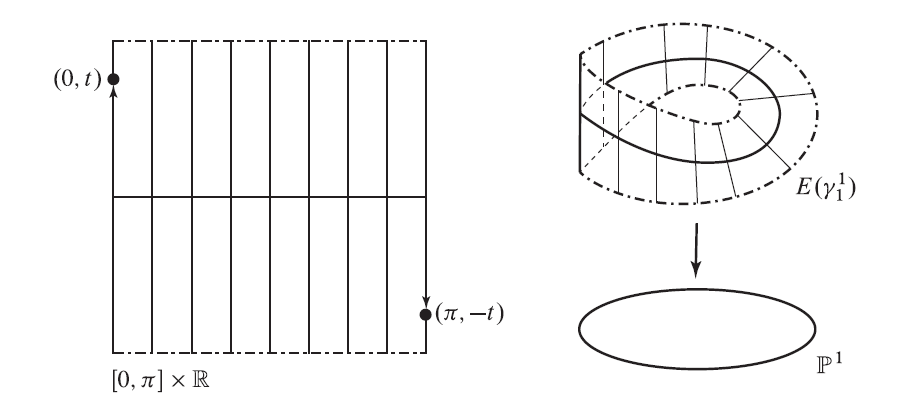
\includegraphics[scale=0.5]{"../tex from old group/fig2.png"}
    \caption{}
    \label{fig:figure2}
\end{figure}

Now consider a collection $\brc{s_1,\dots,s_n}$ of cross-sections of a vector bundle $\xi$.


\begin{definition}\label{def:02.04}
The cross-sections $s_1, \ldots, s_n$ are \defemph{nowhere dependent}\index{cross-section!\indexline nowhere depndent}
if, for each $b \in {\B}$, the vectors $s_1(b), \ldots, s_n(b)$ are linearly independent.
\end{definition}


\begin{theorem}\label{thm:02.02}
An $\bR^n$-bundle $\xi$ is trivial if and only if $\xi$ admits $n$ cross-sections $s_1(b), \ldots, s_n(b)$ which are nowhere dependent.\index{trivial bundle $\trivialbundle^n$}
\end{theorem}


The proof will depend on the following basic result.


\begin{lemma}\label{lem:02.03}
Let $\xi$ and $\eta$ be vector bundles over ${\B}$ and let
$f: \total(\xi) \varrightarrow{} \total(\eta)$ be a continuous function which maps each vector space $F_{b}(\xi)$ isomorphically onto the corresponding vector space $F_{b}(\eta)$. Then $f$ is necessarily a homeomorphism. Hence $\xi$ is isomorphic to $\eta$. \index{isomorphic (vector bundles)}
\end{lemma}


\begin{proof}
Given any point $b_0 \in {\B}$, choose local coordinate systems
$(U,g)$ for $\xi$ and $(V,h)$ for $\eta$, with $b_{0} \in U \cap V$. Then we must show that the composition
\[(U \cap V) \times \mathbb{R}^{n} \varrightarrow{h\inv \circ f \circ g}(U \cap V) \times \mathbb{R}^{n}\]
is a homeomorphism. Setting
\[h\inv(f(g(b, x))) = (b, y)\]
it is evident that $y = \brc{y_1,\ldots,y_n}$ can be expressed in the form
\[y_{i} = \sum_{j} f_{i j}(b) x_{j}\]
where $[f_{i j}(b)]$ denotes a non-singular matrix of real numbers. 
Furthermore, the entries $f_{i j}(b)$ depend continuously on $b$. Let $[F_{ji}(b)]$ denote
the inverse matrix. Evidently
\[(g\inv \circ f\inv \circ h)(b, y) = (b, x), \]
where
\[x_{j} = \sum_{i} F_{ji}(b) y_{i}\]
Since the numbers $F_{ji}(b)$ depend continuously on the matrix $[f_{i j}(b)]$,
they depend continuously on $b$. Thus $g\inv \circ f\inv \circ h$ is continuous, which
completes the proof of \ref{lem:02.03}.
\end{proof}


\begin{proof}[Proof of \ref{thm:02.02}.]
Let $s_1,\ldots,s_n$ be cross-sections of $\xi$ which
are nowhere linearly dependent. Define
$f: {\B} \times \bR^{n} \varrightarrow{} \total$ by
\[f(b, x) = x_{1} s_{1}(b)+\cdots+x_{n} s_{n}(b)\]
Evidently $f$ is continuous and maps each fiber of the trivial bundle $\trivialbundle^n_{\B}$
isomorphically onto the corresponding fiber of $\xi$. Hence $f$ is a bundle
isomorphism, and $\xi$ is trivial.

Conversely suppose that $\xi$ is trivial, with coordinate system $(B, h)$. Defining
\[s_{i}(b) = h(b,(0, \dots, 0,1,0, \dots, 0)) \in F_{b}(\xi)\]
(with the $1$ in the $i$-th place), it is evident that $s_1,\dots,s_n$ are nowhere
dependent cross-sections. This completes the proof.
\end{proof}


As an illustration, the tangent bundle of the circle $S^{1} \subset \bR^2$ admits
one nowhere zero cross-section, as illustrated in Figure \ref{fig:figure3}. (The indicated
arrows lead from $x\in S^{1}$  to $x + v$, where $s(x) = (x, v) = ((x_1,x_2), (-x_2,x_1))$.)
Hence $S^{1}$  is parallelizable\index{parallelizable}. Similarly the $3$-sphere $S^{3}\subset\bR^4$ admits
three nowhere dependent vector fields $s_{i}(x)=(x, \xoverline{s}_{i}(x))$ where
\begin{align*}
		\xoverline{s}_{1}(x)&=(-x_{2}, x_{1},-x_{4}, x_{3}), \\
		\xoverline{s}_{2}(x)&=(-x_{3}, x_{4}, x_{1},-x_{2}), \\
		\xoverline{s}_{3}(x)&=(-x_{4},-x_{3}, x_{2}, x_{1}).
\end{align*}
Hence $S^{3}$ is parallelizable. (These formulas come from the quaternion\index{quaternions $\mathbb{H}$} multiplication in $\bR^4$. Compare \cite{steenrodwhitehead1951}.)

\begin{figure}[ht]
    \centering
    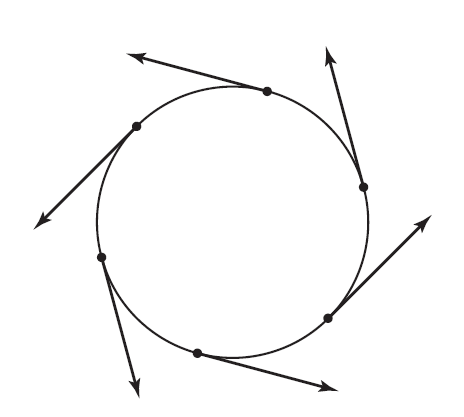
\includegraphics[scale=0.5]{"../tex from old group/fig3.png"}
    \caption{}
    \label{fig:figure3}
\end{figure}

\end{document}